\documentclass[12pt,oneside]{exam}

% This package simply sets the margins to be 1 inch.
\usepackage[margin=1in]{geometry}

% These packages include nice commands from AMS-LaTeX
\usepackage{amssymb,amsmath,amsthm,amsfonts,latexsym,verbatim,xspace,setspace}
\usepackage{hyperref}
\usepackage{graphicx}

% Make the space between lines slightly more
% generous than normal single spacing, but compensate
% so that the spacing between rows of matrices still
% looks normal.  Note that 1.1=1/.9090909...
\renewcommand{\baselinestretch}{1.1}
\renewcommand{\arraystretch}{.91}

% Define environments for exercises.
\newenvironment{exercise}[1]{\vspace{.1in}\noindent\textbf{Exercise #1 \hspace{.05em}}}{}
\newenvironment{newsolution}{\vspace{.1in}\noindent\textbf{Solution: \hspace{.05em}}}{}

% define shortcut commands for commonly used symbols
\newcommand{\R}{\mathbb{R}}
\newcommand{\C}{\mathbb{C}}
\newcommand{\Z}{\mathbb{Z}}
\newcommand{\Q}{\mathbb{Q}}
\newcommand{\N}{\mathbb{N}}
\newcommand{\calP}{\mathcal{P}}
\DeclareMathOperator{\sech}{sech}
\DeclareMathOperator{\csch}{csch}
\DeclareMathOperator{\vsspan}{span}

\title{Math 203 - Summer I 2020: Solutions to Homework 2}

%%%%%%%%%%%%%%%%%%%%%%%%%%%%%%%%%%%%%%%%%%

\begin{document}

\begin{flushright}
\sc MAT 203 - Summer I 2020\\
June 9, 2020
\end{flushright}
\bigskip
 
\begin{center}
\textsf{Homework 2 solutions} 
\end{center}

%%%%%%%%%%%%%%%%%%%%%%%%%%%%%%%%%%%%%%%%

\begin{exercise}{1}
Sketch the curve given by the vector valued function 
\begin{equation*}
r(t)=(t+2,t^2-1)
\end{equation*}
and give the orientation of the curve.
\end{exercise}

\begin{newsolution} 
A plot of the solution, for values of $t$ between $-5$ and $5$ is included below. As t increases, the curve is traversed from left to right. 
\begin{center}
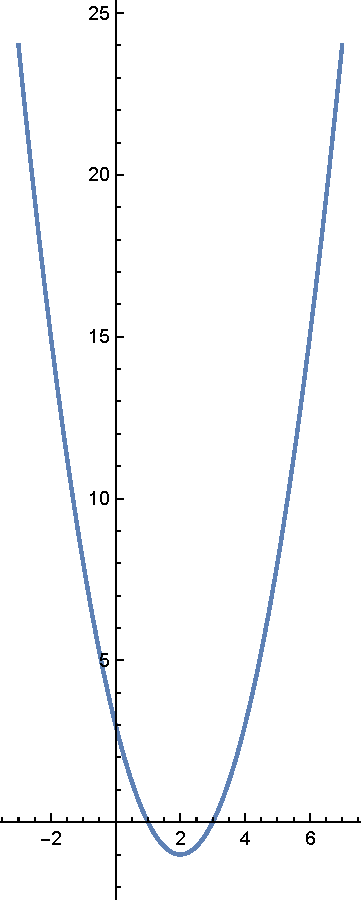
\includegraphics[scale=0.5]{p1.pdf}
\end{center}
\end{newsolution}

\begin{exercise}{2}
Sketch the curve given by the vector valued function
\begin{equation*}
r(t) = 2cos(t)\mathbf{i} + t\mathbf{j} + 2sin(t)\mathbf{k}
\end{equation*}
and give the orientation of the curve.
\end{exercise}

\begin{newsolution}
A plot of the solution, for values of $t$ between $-2\pi$ and $2\pi$ is included below. As t increases, the curve is traversed from left to right, in clockwise sense with respect to the xy-plane. 
\begin{center}
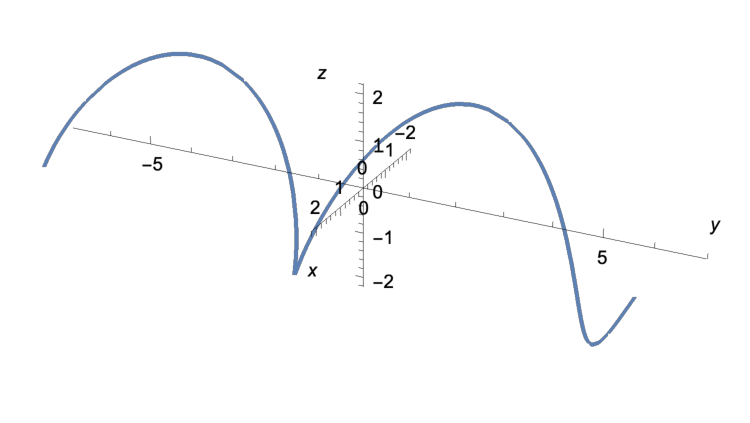
\includegraphics[scale=0.8]{p2.pdf}
\end{center}
\end{newsolution}


\begin{exercise}{3}
Find the limit
\begin{equation*}
\lim_{t \to 0} \frac{sin(2t)}{t}\mathbf{i} + e^{-t}\mathbf{j} + 4\mathbf{k}
\end{equation*}
\end{exercise}

\begin{newsolution}
This limit can be computed component-wise, 
\begin{align*}
\lim_{t \to 0} \frac{\sin(2t)}{t}\mathbf{i} + e^{-t}\mathbf{j} + 4\mathbf{k} & =  \left( \lim_{t \to 0} \frac{\sin(2t)}{t}\right) \mathbf{i} + \left( \lim_{t \to 0} e^{-t}\right) \mathbf{j} + \left( \lim_{t \to 0} 4\right) \mathbf{k} \\
& = 2\mathbf{i} + \mathbf{j} + 4\mathbf{k}.
\end{align*}
\end{newsolution} 

\begin{exercise}{4}
Given 
\begin{equation*}
r(t) = \sin(t)\mathbf{i}+ \cos(t)\mathbf{j} + t\mathbf{k}, \ \ \mbox{and} \ \ u(t) = \sin(t)\mathbf{i} + \cos(t)\mathbf{j} + t^{-1}\mathbf{k},
\end{equation*}
find
\begin{parts}
\part $r'(t)$;
\part $\frac{d}{dt} [u(t)-2r(t)]$;
\part $\frac{d}{dt} [(3t)r(t)]$;
\part $\frac{d}{dt} [r(t)\cdot u(t)]$;
\part $\frac{d}{dt} [r(t) \times u(t)]$;
\part $\frac{d}{dt} [u(2t)]$.
\end{parts}
\end{exercise}

\begin{newsolution}
\begin{parts}
\part $r'(t) = \cos(t)\mathbf{i} - \sin(t)\mathbf{j} + \mathbf{k}$.
\part 
\begin{align*}
\frac{d}{dt} [u(t)-2r(t)] & = u'(t)-2r'(t) \\
& = \cos(t) \mathbf{i} -\sin(t)\mathbf{j} -\frac{1}{t^2}\mathbf{k} -2(\cos(t)\mathbf{i} - \sin(t)\mathbf{j} + \mathbf{k}) \\
& = \cos (t)\mathbf{i} + \sin (t)\mathbf{j} + \left(-\frac{1}{t^2}-2\right)\mathbf{k}
\end{align*}
\part Using the product rule for scalar multiplication,
\begin{align*}
\frac{d}{dt} [(3t)r(t)] & = 3r(t) + 3tr'(t) \\
& = 3\sin(t)\mathbf{i}+ 3\cos(t)\mathbf{j} + 3t\mathbf{k} + 3t(\cos(t)\mathbf{i} - \sin(t)\mathbf{j} + \mathbf{k}) \\
& = (3 \sin(t)+3t\cos(t))\mathbf{i} +(3\cos(t)-3t\sin(t))\mathbf{j} +6 t\mathbf{k}
\end{align*}
\part Using the product rule for the dot product,
\begin{align*}
\frac{d}{dt}(r(t)\cdot u(t)) & = r'(t)\cdot u(t) + r(t) \cdot u'(t) \\
& = (\cos(t),-\sin(t),1) \cdot (\sin(t),\cos(t),t^{-1}) \\
& \ \ \ \ + (\sin(t),\cos(t),t)\cdot (\cos(t),-\sin(t),-t^{-2}) \\
& = \cos(t)\sin(t)-\sin(t)\cos(t)+t^{-1}+\sin(t)\cos(t)-\cos(t)\sin(t)-t^{-1} \\
& = 0
\end{align*}
\part Using the product rule for the cross-product, 
\begin{align*}
\frac{d}{dt} (r(t) \times u(t)) & = r'(t)\times u(t) + r(t) \times u'(t) \\
& = (\cos(t)\mathbf{i}-\sin(t)\mathbf{j}+\mathbf{k}) \times (\sin(t)\mathbf{i}+\cos(t)\mathbf{j}+t^{-1}\mathbf{k}) \\
& \ \ \ \ + (\sin(t)\mathbf{i}+\cos(t)\mathbf{j}+ t\mathbf{k}) \times (\cos(t)\mathbf{i}-\sin(t)\mathbf{j}-t^{-2}\mathbf{k})\\
& = (-t^{-1}\sin(t)-\cos(t))\mathbf{i}-(t^{-1}\cos(t)-\sin(t))\mathbf{j}+\mathbf{k} \\
& \ \ \ \ + (-t^{-2}\cos(t)+t\sin(t))\mathbf{i}-(-t^{-2}\sin(t)-t\cos(t))\mathbf{j}-\mathbf{k} \\
& = \left(\left(t-\frac{1}{t}\right) \sin (t)-\left(1+\frac{1}{t^2}\right) \cos
   (t)\right)\mathbf{i} \\
&  \ \ \ \ + \left(\left(\frac{1}{t^2}+1\right) \sin (t)+\left(t-\frac{1}{t}\right) \cos (t)\right)\mathbf{j}
\end{align*}
\part Using the Chain Rule, 
\begin{equation*}
\frac{d}{dt}u(2t)  = 2 \cos(2t)\mathbf{i} -2 \sin (2 t) \mathbf{j} -\frac{1}{2 t^2}\mathbf{k}.
\end{equation*}

\end{parts}
\end{newsolution}

\begin{exercise}{5}
Sketch the plane curve given by 
\begin{equation*}
r(t) = t^2 \mathbf{i} + 2t \mathbf{j}, 
\end{equation*}
for t between 0 and 3 (inclusive). Find its arclength. 
\end{exercise}

\begin{newsolution}
A plot of the curve is represented below:
\begin{center}
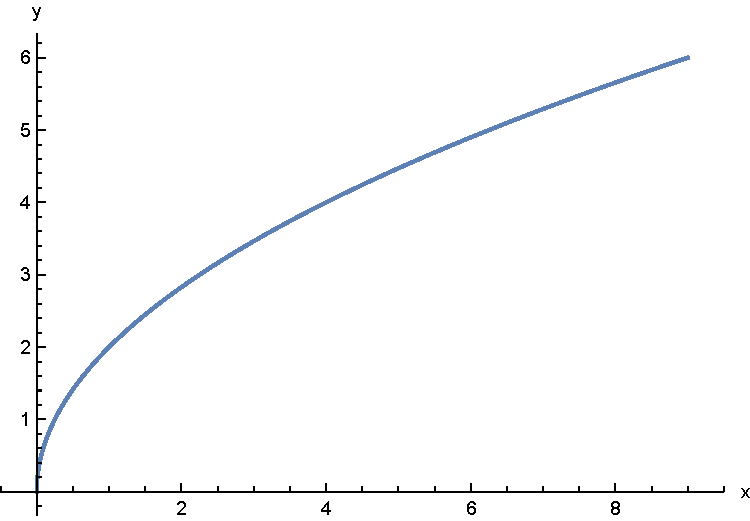
\includegraphics[scale=0.5]{p6.pdf}
\end{center}

The velocity vector of the curve is of the form
\begin{equation*}
r'(t) = 2t\mathbf{i} + 2\mathbf{j}.
\end{equation*}
It follows the arclength is 
\begin{align*}
\int_{0}^{3} \| r'(t)\| dt & = \int_{0}^{3} \sqrt{4t^2+4} \, dt \\
& = 2\int_{0}^{3} \sqrt{t^2+1} \, dt
\end{align*}

There are two ways of solving this integral. The first, more elementary, consists of using a trigonometric substitution $u = \tan(\theta)$. This leads to a long computation involving $\int \sec^3(\theta) \, d\theta$, and we shall not pursue this route here. The second, method makes use of hyperbolic trigonometric functions, and is considerably simpler. We describe the latter alternative in detail below.

Recall that the hyperbolic trigonometric functions $\sinh(x), \cosh(x)$ are defined as 
\begin{align*}
\sinh(x) & = \frac{e^{x}+e^{-x}}{2}, \\
\cosh(x) & = \frac{e^{x}-e^{-x}}{2},
\end{align*}
with other functions $\tanh(x), \sech(x), \csch(x), \coth(x)$ being defined by ratios, similarly to their trigonometric counterparts. 

The key properties we will use to solve this problem are the hyperbolic version of the Fundamental Theorem of Trigonometry, 
\begin{equation*}
\cosh^2(x)-\sinh^2(x) = 1,
\end{equation*}
or, in the form we are most interested in
\begin{equation*}
\cosh^2(x) = 1 + \sinh^2(x),
\end{equation*}
and the relations between derivatives of the hyperbolic functions, 
\begin{equation*}
\frac{d}{dx}\sinh(x) = \cosh(x), \, \frac{d}{dx}\cosh(x) = \sinh(x).
\end{equation*}
A substitution $t = \sinh(x)$ now yields
\begin{align*}
\int \sqrt{t^2+1} \, dt & = \int \left(\sqrt{\sinh^2(x)+1}\right)\cosh(x) \, dx \\
& = \int \cosh^2(x) \, dx \\
& = \int \frac{e^{2x}+2+e^{-2x}}{4} \, dx \\
& = \frac{1}{4} \left( \frac{e^{2x}}{2}+2x -\frac{e^{-2x}}{2} \right) + C \\
& = \frac{1}{4}\left( \frac{e^{2x}}{2}-\frac{e^{-2x}}{2} \right) + \frac{x}{2}  + C\\
& = \frac{1}{2}\left( \frac{e^{x}+e^{-x}}{2}\right)\left(\frac{e^{x}-e^{-x}}{2} \right) + \frac{x}{2}+C\\
& = \frac{\cosh(x)\sinh(x)}{2}+\frac{x}{2}+C\\
& = \frac{t\sqrt{t^2+1}}{2} + \frac{\sinh^{-1}(t)}{2} + C.
\end{align*}
By evaluating this antiderivative at the endpoints of the integral, we obtain
\begin{equation*}
\int_{0}^{3} \| r'(t)\| dt = 2\int_{0}^{3} \sqrt{t^2+1} \, dt = \left[ t\sqrt{t^2+1}+ \sinh^{-1}(t) + C \right] \Big|_{0}^{3} =  3 \sqrt{10}+\sinh ^{-1}(3).
\end{equation*}
\end{newsolution}. 

\begin{exercise}{6}
Find the domain and range of the function
\begin{equation*}
f(x,y) = \sqrt{36 - x^2-y^2}
\end{equation*}
\end{exercise}

\begin{newsolution}
The square-root function is defined so long as its argument is non-negative, thus the domain of $f$ consists of the points in the plane satisfying this constraint
\begin{equation*}
\mathrm{Dom}(f) =\{ (x,y) \in \mathbb{R}^2 | x^2+y^2 \leq 36\}.
\end{equation*}
The range of values attained by this function is $\mathrm{Ran}(f) = [0,6]$. Below is a plot of the graph of the function (this is not necessary and will not contribute towards your grade).
\begin{center}
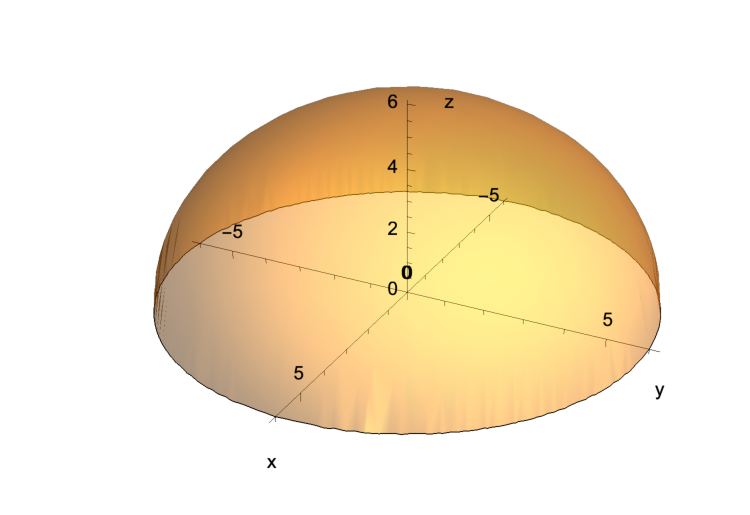
\includegraphics[scale=0.8]{p3.pdf}
\end{center}
\end{newsolution}

\begin{exercise}{7}
Describe the level curves of the function
\begin{equation*}
f(x,y) = 2x^2+y^2.
\end{equation*}
Sketch the surface
\begin{equation*}
z = 2x^2+y^2
\end{equation*}
using level curves for the following c-values: $1, 2, 3, 4, 5$. 
\end{exercise}

\begin{newsolution}
The level curves satisfy 
\begin{equation*}
2x^2 + y^2 = c.
\end{equation*}
As the left-hand side is a sum of non-negative numbers, the level set is empty for negative values of $c$, and consists of a singule point, the origin, when $c=0$. Meanwhile, for positive values of $c$, the level set describes an elipse. Below is a contour plot for this function, displaying several level sets.
\begin{center}
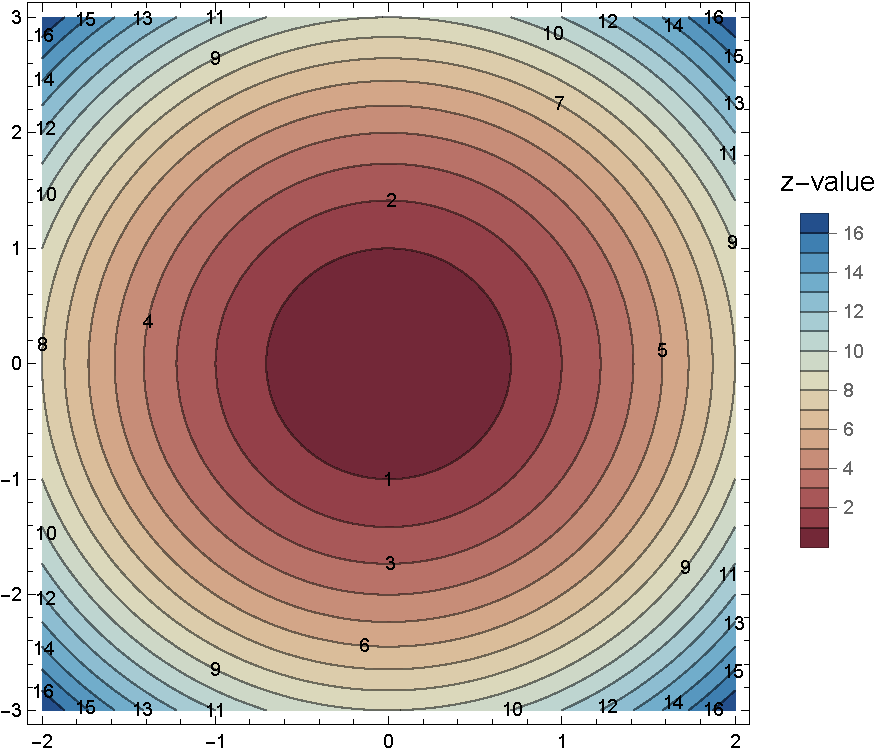
\includegraphics[scale=0.5]{p4.pdf}
\end{center}
Next we sketch the surface, overlaying several level sets.
\begin{center}
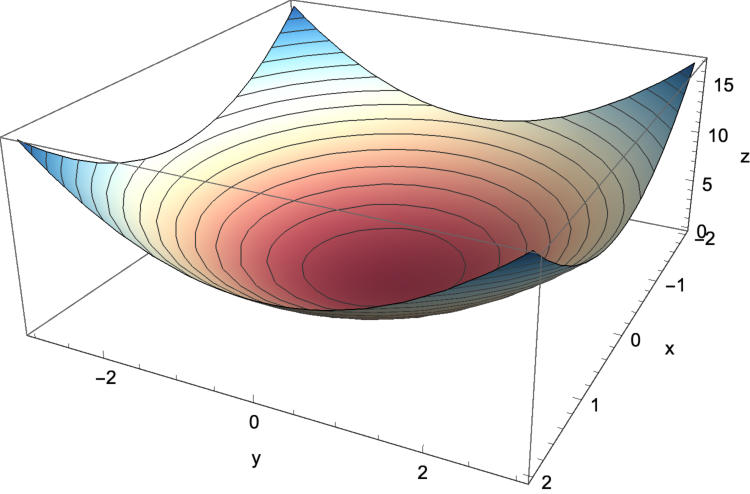
\includegraphics[scale=0.5]{p5.pdf}
\end{center}
\end{newsolution}

\begin{exercise}{8}
Find the limit, if it exists, and discuss the continuity of the function
\begin{equation*}
\lim_{(x,y) \to (1,1)} \frac{xy}{(x^2-y^2)}
\end{equation*}
\end{exercise}

\begin{newsolution}
This limit does not exist. Indeed, examining the lateral limits of expression along the line $x=1$, we obtain
\begin{equation*}
\lim_{y \to 1-} \frac{y}{(1-y^2)} = \infty,
\end{equation*}
while
\begin{equation*}
\lim_{y \to 1+} \frac{y}{(1-y^2)} = -\infty,
\end{equation*}

This function is continuous wherever the denominator is non-zero, that is, on
\begin{equation*}
\mathrm{Dom}(f) = \{(x,y) \in \mathbb{R}^2 | x\neq \pm y \}.
\end{equation*}
\end{newsolution}

\begin{exercise}{9}
Find the limit, if it exists, and discuss the continuity of the function
\begin{equation*}
\lim_{(x,y)\to(0,0)} \frac{x^2y}{(x^4+y^2)}.
\end{equation*}
\end{exercise}

\begin{newsolution}
Consider the limits along parabolae $y=kx^2$,
\begin{align*}
\lim_{x \to 0} \frac{x^2(kx^2)}{(x^4+(kx^2)^2)} & = \lim_{x \to 0} \frac{kx^4}{(1+k^2)x^4}\\
& = \frac{k}{1+k^2}. 
\end{align*}
Since limits along such parabolae depend on the value of $k$, the multivariable limit of the function does not exist. 
\end{newsolution}

\begin{exercise}{10} 
Find all first partial derivatives of the function
\begin{equation*}
f(x,y,z) = 2xz^2 + 6xyz.
\end{equation*}
\end{exercise}

\begin{newsolution}
The derivatives are as follows:
\begin{align*}
\partial_{x}f & = 2z^2+6yz \\
\partial_{y}f & = 6xz \\
\partial_{z}f & = 4xz+6xy.
\end{align*}
\end{newsolution}


\begin{exercise}{11}
Find the four second partial derivatives of the function
\begin{equation*}
g(x,y) = \cos(x-2y).
\end{equation*}
Observe that the mixed partials are equal.
\end{exercise}

\begin{newsolution}
We begin with the computation of first partials, 
\begin{align*}
\partial_x g & = -\sin(x-2y),\\
\partial_y g & = 2\sin(x-2y).
\end{align*}
From these we compute the second partials, 
\begin{align*}
\partial_{xx} g & = -\cos(x-2y),\\
\partial_{xy} g & = 2\cos(x-2y),\\
\partial_{yx} g & = 2\cos(x-2y),\\
\partial_{yy} g & = -4\cos(x-2y).
\end{align*}
\end{newsolution}


\begin{exercise}{12}
You are given functions satisfying 
\begin{equation*}
w=x^2+y^2+z^2, \,  x=r\cos(t)  \,  y=r\sin(t) \, z=t.
\end{equation*}
Find the partial derivatives of w relative to r and t, by
\begin{parts}
\part using the appropriate Chain Rule, and;
\part converting w to a function of r and t before differentiating. 
\end{parts}
\end{exercise}

\begin{newsolution}
\begin{parts}
\part By the Chain Rule, 
\begin{align*}
\frac{\partial w}{\partial r} & = 2x\frac{\partial x}{\partial r} + 2y\frac{\partial y}{\partial r} + 2z \frac{\partial z}{\partial r} \\
& = 2r\cos(t)\cdot \cos(t)+2r\sin(t)\cdot \sin(t) +2t\cdot 0\\
& = 2r[\cos^2(t)+\sin^2(t)]\\
& =2r.
\end{align*}
Similarly, 
\begin{align*}
\frac{\partial w}{\partial t} & = 2x\frac{\partial x}{\partial t} + 2y\frac{\partial y}{\partial t} + 2z\frac{\partial z}{\partial t} \\
& = 2r\cos(t)(-r\sin(t)) + 2r\sin(t)(r\cos(t))+2t\\
& = 2t
\end{align*}
\part By direclty substituting $x,y$ and $z$ into the equation defining $w$, we have 
\begin{equation*}
w = r^2\cos^2(t) + r^2\sin^2(t) + t^2 = r^2+t^2
\end{equation*}
hence it follows easily that the derivatives can be written as 
\begin{equation*}
\frac{\partial w}{\partial r} = 2r, \, \frac{\partial w}{\partial t} = 2t.
\end{equation*}
\end{parts}
\end{newsolution}

\end{document}

